\documentclass[conference]{IEEEtran}
\IEEEoverridecommandlockouts

\usepackage[T1]{fontenc}
\usepackage[utf8]{inputenc}
\usepackage{microtype}
\usepackage{amsmath,amssymb}
\usepackage{booktabs,array,tabularx}
\usepackage{graphicx,xcolor}
\usepackage{tikz}
\usetikzlibrary{arrows.meta,positioning,fit,calc}
\usepackage{cite}
\usepackage{url}
\usepackage[hidelinks]{hyperref}

\newcolumntype{Y}{>{\raggedright\arraybackslash}X}
\newcommand{\FPR}{\mathrm{FPR}}
\newcommand{\FNR}{\mathrm{FNR}}
\DeclareMathOperator*{\argmin}{arg\,min}
\def\BibTeX{{\rm B\kern-.05em{\sc i\kern-.025em b}\kern-.08em T\kern-.1667em\lower.7ex\hbox{E}\kern-.125emX}}

\makeatletter
\def\bstctlcite{\@ifnextchar[{\@bstctlcite}{\@bstctlcite[@auxout]}}
\def\@bstctlcite[#1]#2{\@bsphack\@for\@citeb:=#2\do{\edef\@citeb{\expandafter\@firstofone\@citeb}\if@filesw\immediate\write\csname #1\endcsname{\string\citation{\@citeb}}\fi}\@esphack}
\def\abstract{\normalfont\@IEEEabskeysecsize\bfseries\textit{\abstractname}\ -\ \relax\@IEEEgobbleleadPARNLSP}
\def\IEEEkeywords{\normalfont\@IEEEabskeysecsize\bfseries\textit{\IEEEkeywordsname}\ -\ \relax\@IEEEgobbleleadPARNLSP}
\makeatother

\begin{document}
\bstctlcite{IEEEexample:BSTcontrol}

\title{Evaluating Password Strength Meters Against Simulated Guessing Attackers: Human, Random and AI-Generated Passwords}

\author{%
\IEEEauthorblockN{AINOUCHE Rayan (N\textordmasculine{} 145882), JOVANOVIC Marko (N\textordmasculine{} 145885),\\GERMAIN Valentine (N\textordmasculine{} 146069), ADYEL Ilyes (N\textordmasculine{} 145869)}
\IEEEauthorblockA{Iscte - Instituto Universit\'ario de Lisboa\\
Network and Information Systems Security - Prof.\ Jos\'e Andr\'e Moura}}

\maketitle

\begin{abstract}
Password strength meters (PSMs) decide, at password-creation time, whether a password is good enough. A meter that rates a guessable password ``strong'' gives users false confidence. Earlier studies compare meters with simulated attackers, but, to our knowledge, none reports how often meters accept guessable passwords for human, random and large-language-model (LLM) generated passwords together, and none includes the Linux password-quality tools \texttt{libpwquality} and \texttt{passwdqc}. This paper is the theoretical part of our project. We review the state of the art and specify a protocol that measures the \emph{dangerous false-positive rate}, the share of guessable passwords that a meter rates strong, for five meters (zxcvbn, composition rules, \texttt{libpwquality}, \texttt{passwdqc}, Have I Been Pwned). Ground truth is the minimum guess number over simulated attackers (dictionary, rule-based, LLM-aware) up to $10^{10}$ guesses. Pilot measurements show that the protocol is feasible on a 2-core machine: a $10^{10}$-guess rule-based stream takes about 41 minutes, and a first end-to-end run with a dictionary attacker already separates the meters. Results are left to the practical part.
\end{abstract}

\begin{IEEEkeywords}
password strength meter, guessability, zxcvbn, Have I Been Pwned, large language models
\end{IEEEkeywords}

%% =====================================================================
\section{Introduction}
Passwords remain the default authentication mechanism, and users choose them under the guidance of password strength meters: composition-rule checkers, strength bars, or blocklist checks. A meter is only useful if its verdict matches real strength; in the words of Golla and D\"urmuth, ``a strength meter with low accuracy may do more harm than good''~\cite{golla2018}. The harm is asymmetric. Rating a weak password strong gives false confidence, whereas rating a strong password weak mainly annoys the user~\cite{wang2023}.

Two developments motivate this work. First, NIST SP~800-63B-4 (July 2025) requires verifiers to compare new passwords with a blocklist of commonly used, expected or compromised passwords, and forbids other composition rules~\cite{nist80063b4}, while Golla and D\"urmuth found composition-based (LUDS) meters, with poor accuracy, in several password managers and operating systems~\cite{golla2018}. Second, users and coding assistants now ask LLMs to generate passwords. Irregular reports that 50 runs of one model produced only 30 distinct 16-character passwords, one of them 18 times, and estimates about 27 bits of entropy for such a password against about 98 bits for a random one; it also reports that KeePass and zxcvbn rated the password as very strong (about 100 bits, ``centuries'')~\cite{irregular2026}. This is a small, single-vendor case study, not a measurement against attackers.

\textbf{Problem.} How often do common meters accept passwords that a realistic attacker would guess, and does the answer depend on who or what created the password? We answer with guessability-based evaluation, now the standard method~\cite{wheeler2016,golla2018,wang2023}: simulate attackers, compute a guess number for each test password, and compare it with the meter's verdict.

\textbf{Research questions.}
\begin{itemize}
\item \textbf{RQ1.} For each meter and each population (human, random, LLM), what share of the passwords guessed within a budget $\theta$ is rated strong (dangerous false positives)?
\item \textbf{RQ2.} Does this share differ between populations, in particular for LLM passwords attacked by an LLM-aware attacker?
\item \textbf{RQ3.} What does each meter cost in usability (strong passwords rejected), and how do both errors change with $\theta$?
\end{itemize}

\textbf{Contributions.} (C1) A comparison of eight related works along the dimensions that matter for our question (Sec.~\ref{sec:related}). (C2) A protocol with explicit definitions, equations and design choices justified by the literature (Sec.~\ref{sec:method}). (C3) Pilot measurements of throughput, redundancy and an end-to-end smoke test showing that the protocol is feasible (Sec.~\ref{sec:feasibility}). (C4) A nine-week plan, a repository structure and a list of threats to validity.

%% =====================================================================
\section{Background and Related Work}\label{sec:related}

\subsection{Guess numbers and ground truth}
The \emph{guess number} of a password $p$ for an attacker $A$ is the position at which the attacker's ordered candidate list first contains $p$ (Eq.~\ref{eq:gn}). Ur et al.\ compared guessing tools and found that running a single algorithm often gives a very poor estimate of strength; they therefore propose the minimum over several configured attacks (\emph{min\_auto}), which the CMU Password Guessability Service provides~\cite{ur2015,golla2018}. Wheeler takes the minimum over four attacks (PCFG, Markov, hashcat, John the Ripper) as ground truth~\cite{wheeler2016}; Wang et al.\ use the union of three attacks~\cite{wang2023}. For probabilistic models, guess numbers beyond what can be enumerated can be estimated by Monte Carlo sampling~\cite{dellamico2015}, which Wang et al.\ use to convert probabilities into guess numbers~\cite{wang2023}.

Training data matter. Wang et al.\ require that training and test sets never come from the same service~\cite{wang2023}; Wheeler notes that his same-distribution split makes the simulated attacker aggressive~\cite{wheeler2016}. Xu et al.\ (arXiv preprint) show that data-driven meters over-learn their training passwords, which then receive unusually high probabilities and can be recovered by membership inference~\cite{xu2025}.

\subsection{Meter families and standards}
\emph{Composition-rule (LUDS) meters} count lower-case and upper-case letters, digits and symbols. Golla and D\"urmuth measured them as inaccurate: the weighted Spearman correlation of Comprehensive8 with the reference is negative on RockYou and LinkedIn (online: -0.652 and -0.589; offline: -0.476 and -0.616)~\cite{golla2018}. \emph{Pattern-based estimators} such as zxcvbn match dictionary words, keyboard patterns, sequences, repeats and dates and estimate a guess count~\cite{wheeler2016}; Wang et al.\ map such counts to zxcvbn-style scores with thresholds $10^3, 10^6, 10^8, 10^{10}$~\cite{wang2023}. \emph{Blocklists} are mandatory in NIST SP~800-63B-4, which compares the \emph{entire} password with a list of breached, dictionary and context-specific words and asks verifiers to explain a rejection~\cite{nist80063b4}. Have I Been Pwned (HIBP) exposes such a list through a k-anonymity range API: the client sends the first five hexadecimal characters of the SHA-1 hash and receives the matching suffixes with their counts~\cite{hibp}. Golla and D\"urmuth rank it among the most accurate meters (weighted Spearman 0.739-0.997) but note that this is probably due to the tested leaks being part of the list~\cite{golla2018}. \texttt{libpwquality} and \texttt{passwdqc} are the password-quality libraries behind Linux PAM modules~\cite{pwquality,passwdqc}; they are not among the meters evaluated by Golla and D\"urmuth or by Wang et al.

\subsection{Measuring accuracy}
\emph{Wheeler} measures, in orders of magnitude, the gap between a meter's estimate and the ground-truth guess number on 15\,k RockYou passwords. Below $10^6$ guesses, zxcvbn's mean absolute error is 0.58 orders of magnitude (version with 100\,k-token dictionaries), against 1.81 for a NIST-entropy estimator and 1.43 for KeePass; above $10^6$ it grows to 2.20. Wheeler therefore presents the tool as accurate and conservative at low magnitudes, suited to online attacks~\cite{wheeler2016}.

\emph{Golla and D\"urmuth} test 19 similarity measures against five requirements and select the weighted Spearman correlation, with password frequency as weight; they compare 45 meters (81 variants) on RockYou, LinkedIn and 000Webhost, using sample frequency (top $10^4$ pool) as online reference and PGS min\_auto as offline reference~\cite{golla2018}. They acknowledge that the measure does not distinguish under- from over-estimation and that quantized meters must be interpreted with care~\cite{golla2018}.

\emph{Wang et al.}\ propose four metrics: weighted Spearman (online, threshold $10^4$ guesses), KL divergence, Precision and PrecisionSecurity (offline, above $10^9$ guesses), over 12 meters and 7 English and 7 Chinese leaks, with training and test sets from different services~\cite{wang2023}. PrecisionSecurity weights weak$\to$strong errors with $\beta=0.8$, but, as printed, its $\beta$-weighted term is computed on the lowest-score set $L$, whereas weak$\to$strong errors are the cracked passwords in the highest-score set $H$. We therefore measure the weak$\to$strong error directly (Eq.~\ref{eq:fpr}).

\emph{Tan et al.}\ run two MTurk experiments (4{,}317 and 4{,}005 participants completed password creation) comparing blocklists, minimum-strength requirements and composition rules, with guessability from PGS min\_auto at $10^6$ (online) and $10^{14}$ (offline) guesses; they recommend blocklists or minimum-strength requirements and advise against character-class requirements~\cite{tan2020}.

\subsection{Which budgets matter}
Flor\^encio et al.\ argue that guessing resistance matters only below an online limit $T_0\approx10^6$ and above an offline limit $T_1\approx10^{14}$; between them lies a ``don't care'' region, and they favour blacklists, throttling and hash iteration over composition policies~\cite{florencio2016}. Golla and D\"urmuth cite 100-1000 online guesses per 30 days and $10^9$-$10^{12}$ offline guesses per day on one GPU~\cite{golla2018}. Our budget $B=10^{10}$ lies inside the ``don't care'' region; Sec.~\ref{sec:method} explains why we still use it.

\subsection{LLM-generated passwords}
Beyond the Irregular report~\cite{irregular2026} (a company blog post, not peer-reviewed), Atzori et al.\ (arXiv preprint) study LLMs that generate and evaluate passwords from social-profile data for 100 users; they rely on their own composite metric (CPS) and report that 22 of 25{,}000 strong generated passwords were found by a targeted guesser~\cite{atzori2025}. Neither work simulates attackers against standard meters.

\subsection{Comparison and gap}
Table~\ref{tab:related} summarizes the works. None combines (i) Linux password-quality tools, (ii) a threshold-based, one-sided error measure for accept/reject verdicts, and (iii) human, random and LLM-generated passwords with an attacker that knows the LLM output distribution. Golla and D\"urmuth note that their selected measure does not distinguish under- from over-estimation and that quantized outputs need careful interpretation~\cite{golla2018}; a one-sided error for binary verdicts is what we add.

\begin{table*}[t]
\centering
\caption{Comparison of related work. ``Budget'' is the number of guesses of the ground-truth attacker.}
\label{tab:related}
\footnotesize
\renewcommand{\arraystretch}{1.15}
\begin{tabularx}{\textwidth}{@{}l Y Y Y Y c@{}}
\toprule
\textbf{Work} & \textbf{Meters evaluated} & \textbf{Ground truth (budget)} & \textbf{Passwords} & \textbf{Main metric} & \textbf{LLM}\\
\midrule
Wheeler 2016~\cite{wheeler2016} & zxcvbn, NIST entropy, KeePass & min of PCFG, Markov, hashcat, JtR (caps $10^{10}$-$10^{14}$) & 15\,k RockYou (+ Yahoo) & $|\Delta|$, $\Delta^+$ in orders of magnitude & no\\
Golla 2018~\cite{golla2018} & 45 meters (81 variants) & online: frequency, top $10^4$; offline: PGS min\_auto & RockYou, LinkedIn, 000Webhost & weighted Spearman & no\\
Wang 2023~\cite{wang2023} & 12 meters & online $10^4$; offline JtR+rules, Markov, brute force ($10^9$-$10^{12}$), union & 7 English + 7 Chinese leaks; train $\neq$ test service & WSpearman, KL, Precision, PrecisionSecurity & no\\
Tan 2020~\cite{tan2020} & minimum-strength NN, blocklists, composition (user study) & PGS min\_auto; $10^6$ online, $10^{14}$ offline & passwords created by MTurk participants & \% guessed, usability & no\\
Flor\^encio 2016~\cite{florencio2016} & conceptual & $T_0\approx10^6$, $T_1\approx10^{14}$ & none (cites earlier studies) & analytical & no\\
Xu 2025~\cite{xu2025} & 11 meters (risks of the meter itself) & membership inference, meter-aware guessing & six leaks, incl.\ RockYou & MIA F1, accounts compromised & no\\
Irregular 2026~\cite{irregular2026} & KeePass, zxcvbn (informal) & entropy estimates (character statistics, log-probabilities) & 50 runs per LLM & entropy in bits & yes\\
Atzori 2025~\cite{atzori2025} & zxcvbn, CKL\_PSM, semantic PCFG, own tool & targeted guesser (PassBERT); own CPS metric & 100 users' profiles & CPS, accuracy, F1 & yes\\
\midrule
\textbf{This work} & zxcvbn, composition, \texttt{libpwquality}, \texttt{passwdqc}, HIBP & min over dictionary, rules, LLM-aware ($B=10^{10}$) & phpBB, random, LLM & dangerous FPR, FNR & yes\\
\bottomrule
\end{tabularx}
\end{table*}

%% =====================================================================
\section{Problem Statement and Hypotheses}
We evaluate the verdict $V_M(p)\in\{\text{strong},\text{weak}\}$ of each meter $M$ on three populations: human passwords (H), random passwords (R, control) and LLM-generated passwords (L). Targeted attacks, user-behaviour effects and meter feedback text are out of scope.

Our hypotheses are informed by the literature and by the pilot of Sec.~\ref{sec:feasibility}; they are to be tested, not assumed.
\begin{description}
\item[H1] No meter dominates on both errors. Strict meters (composition, \texttt{passwdqc}) will show a low false-positive rate but reject most strong passwords, so FPR must be read together with FNR (the pilot already shows this).
\item[H2] The FPR of zxcvbn rises from the online budget to $B$, because the tool was validated only in the online range~\cite{wheeler2016}. As an order of magnitude, our reading of the cell counts of Fig.~2(b) in~\cite{golla2018} (zxcvbn score against the PGS min\_auto guess number, sample of 10{,}000 passwords) gives 51 of 1{,}108 passwords with score 4 and a guess number below $10^{10}$ (4.6\,\%).
\item[H3] Most LLM samples are rated strong by pattern- and composition-based meters~\cite{irregular2026} while the LLM-aware attacker guesses a large share of them; HIBP rates nearly all of them strong, since fresh LLM output is unlikely to be in breach corpora.
\end{description}

%% =====================================================================
\section{Methodology}\label{sec:method}

Fig.~\ref{fig:pipeline} summarizes the pipeline and Table~\ref{tab:decisions} lists each design decision with its source.

\subsection{Meters under test}
Table~\ref{tab:meters} fixes one binary verdict per meter. For graded meters (zxcvbn guess number, \texttt{pwscore} score) we also sweep the threshold and report FPR against FNR curves.

zxcvbn estimates the guess count of a password as the minimum, over non-overlapping covers $S$ of the password by matched patterns, of~\cite{wheeler2016}
\begin{equation}\label{eq:zx}
\hat g(p)=\min_{S}\Big[\,|S|!\prod_{m\in S} g(m)+D^{|S|-1}\Big],\quad D=10^4,
\end{equation}
where $g(m)$ is the guess estimate of match $m$ (for unmatched characters, $10^{\ell}$ for $\ell$ brute-force characters). The 0-4 score is the number of thresholds exceeded (the thresholds come from the zxcvbn source code, not from~\cite{wheeler2016}),
\begin{equation}\label{eq:zxscore}
s(\hat g)=\sum_{t\in\{10^3,10^6,10^8,10^{10}\}}\mathbf 1\!\left[\hat g\ge t+5\right].
\end{equation}
We checked Eq.~\eqref{eq:zxscore} against the Python package (version 4.5.0) on 2{,}000 random passwords: no mismatch.

\begin{table}[t]
\centering
\caption{Meters and the binary verdict ``strong''.}
\label{tab:meters}
\footnotesize
\renewcommand{\arraystretch}{1.12}
\begin{tabularx}{\columnwidth}{@{}l Y Y@{}}
\toprule
\textbf{Meter} & \textbf{Implementation} & \textbf{Strong iff}\\
\midrule
zxcvbn & Python package 4.5.0, reference year pinned to 2026 (Sec.~\ref{sec:feasibility}) & score $\ge3$ ($\hat g\ge10^8$)\\
Composition & own function & length $\ge8$ and $\ge3$ of 4 classes\\
\texttt{pwscore} & \texttt{libpwquality} tools~\cite{pwquality}, default configuration & password accepted (exit code 0)\\
\texttt{pwqcheck} & \texttt{passwdqc}~\cite{passwdqc}, default configuration & password accepted (exit code 0)\\
HIBP & range API, 5-hex prefix, \texttt{Add-Padding: true}~\cite{hibp} & count $=0$\\
\bottomrule
\end{tabularx}
\end{table}

\subsection{Password populations}
Table~\ref{tab:pop} lists the populations. Attackers are trained on RockYou and tested on a different service (phpBB), as required by~\cite{wang2023}; Wang et al.\ also train on RockYou. Passwords are ASCII, 8-64 characters: 8 is the NIST minimum for passwords used with multi-factor authentication~\cite{nist80063b4}, whereas the 15-character single-factor minimum would keep only 0.18\,\% of the phpBB accounts (463 of 255{,}420). Evaluation is at the \emph{account} level: a password used by $c$ accounts counts $c$ times, so that each observation is an independent draw from the user population. Random passwords are drawn uniformly from the 94 printable non-space ASCII symbols with Python's \texttt{secrets}; their entropy is $L\log_2 94$ bits ($52.4$, $78.7$, $104.9$ bits for $L=8,12,16$). LLM passwords come from three open-weight instruction-tuned models of at most 4~billion parameters, run locally on CPU with Ollama~\cite{ollama} so that generation costs nothing (Sec.~\ref{sec:zerocost}; the list is fixed after the week-1 benchmark), with two prompts: a neutral one (``Please generate a password'', as in~\cite{irregular2026}) and one that asks for a strong 16-character password; each generation is an independent session at temperature 0.7, the value used in~\cite{irregular2026}.

\begin{table}[t]
\centering
\caption{Password populations. Counts for RockYou and phpBB are from the SecLists copies~\cite{seclists} before/after our filter.}
\label{tab:pop}
\footnotesize
\renewcommand{\arraystretch}{1.12}
\begin{tabularx}{\columnwidth}{@{}l Y Y@{}}
\toprule
\textbf{Group} & \textbf{Source} & \textbf{Size / role}\\
\midrule
RockYou & leak, all lengths & 14{,}344{,}391 unique, 32{,}603{,}388 accounts; attacker training only\\
H & phpBB leak, ASCII, 8-64 chars & 95{,}837 unique, 116{,}289 accounts; test\\
R & \texttt{secrets}, 94 symbols, $L\in\{8,12,16\}$ & $3\times10{,}000$; control\\
L-train & LLM, per (model, prompt) & 1{,}000; builds attacker A4\\
L-test & LLM, per (model, prompt) & 1{,}000; test\\
\bottomrule
\end{tabularx}
\end{table}

\subsection{Ground-truth attackers}
For an attacker $A$ producing a candidate stream $(c_1,c_2,\dots)$ truncated at budget $B$,
\begin{equation}\label{eq:gn}
G_A(p)=\begin{cases}\min\{k\le B : c_k=p\} & \text{if } p\in\{c_1,\dots,c_B\},\\ \infty & \text{otherwise.}\end{cases}
\end{equation}
The ground-truth guess number and the label at budget $\theta\le B$ follow the min\_auto principle~\cite{ur2015}:
\begin{equation}\label{eq:gt}
G(p)=\min_{A\in\mathcal A}G_A(p),\qquad y_\theta(p)=\mathbf 1\!\left[G(p)\le\theta\right].
\end{equation}
We compute $G(p)$ once with $B=10^{10}$ and evaluate every $\theta\in\{10^4,10^6,10^8,10^9,10^{10}\}$ afterwards, at no extra cost. The headline budgets are $\theta_{\text{on}}=10^6$ (online limit of~\cite{florencio2016,tan2020}) and $\theta_{\text{off}}=B=10^{10}$; $10^4$ is Wang's online threshold~\cite{wang2023}, $10^8$ and $10^{10}$ are the claims of zxcvbn scores 3 and 4, and $10^9$ is Wang's offline floor. At the rates cited in~\cite{golla2018} ($10^9$-$10^{12}$ guesses per day and GPU), $B$ costs between 15 minutes and 10 GPU-days. We do not reach the $10^{14}$ offline limit of~\cite{florencio2016,tan2020}: enumerating it would take about 285 days at our measured rate. Our guess numbers are therefore upper bounds on strength, and the measured FPR are expected to be lower bounds on the true danger.

\begin{table}[t]
\centering
\caption{Attackers. Cost: measured rate of Sec.~\ref{sec:feasibility} (A2a extrapolated).}
\label{tab:att}
\footnotesize
\renewcommand{\arraystretch}{1.12}
\begin{tabularx}{\columnwidth}{@{}l Y r r@{}}
\toprule
\textbf{ID} & \textbf{Candidates} & \textbf{Budget} & \textbf{Cost}\\
\midrule
A1 & RockYou list by decreasing frequency & $1.4{\times}10^{7}$ & seconds\\
A2a & hashcat~\cite{hashcat} \texttt{best64} (77 rules) on the full list & $1.10{\times}10^{9}$ & $\approx31$ min\\
A2b & hashcat \texttt{dive} (99{,}086 rules) on the top $10^5$ words & $9.91{\times}10^{9}$ & $\approx41$ min\\
A4 & LLM-aware: outputs of the same (model, prompt) in L-train, by decreasing frequency & $\le10^3$ & seconds\\
\bottomrule
\end{tabularx}
\end{table}

Ur et al.\ show that a single default configuration under-estimates guessability~\cite{ur2015}, so A2 uses two configurations and the minimum is kept. A4 knows the model and prompt but not the test samples; for ties in frequency, $G_{A4}$ is the end of the tie group, which is conservative. Hashcat enumerates words in the outer loop and rules in the inner loop, and its streams contain duplicates; $G_A$ is the raw stream position and therefore upper-bounds the deduplicated rank (Sec.~\ref{sec:feasibility}).

Simulated brute force is omitted on purpose. With 94 symbols, the number of passwords of length at most $L$ is
\begin{equation}\label{eq:bf}
N_{BF}(L)=\sum_{k=1}^{L}94^{k}.
\end{equation}
Since $N_{BF}(5)=7.42{\times}10^{9}<B<N_{BF}(6)=6.97{\times}10^{11}$, brute force reaches only lengths $\le5$ within $B$, and all our test passwords have at least 8 characters. The expected guess number of a random 8-character password is $94^8/2\approx3.0{\times}10^{15}\gg B$: random passwords are unguessed by construction, and serve as a control for the meters' strong rate.

\subsection{Metrics}
Let a ``positive'' be a strong verdict. For a population $P$ of accounts and a budget $\theta$:
\begin{align}
\FPR_\theta(M;P)&=\frac{\#\{p\in P:V_M(p)=\text{strong}\wedge y_\theta(p)=1\}}{\#\{p\in P:y_\theta(p)=1\}},\label{eq:fpr}\\
\FNR_\theta(M;P)&=\frac{\#\{p\in P:V_M(p)=\text{weak}\wedge y_\theta(p)=0\}}{\#\{p\in P:y_\theta(p)=0\}}.\label{eq:fnr}
\end{align}
Eq.~\eqref{eq:fpr} is the \emph{dangerous false-positive rate}, our primary metric: it does not depend on how many guessable passwords the population contains, unlike the share of guessed passwords among those rated strong. FNR is the usability cost. Because ground truth under-estimates guessability, FNR is expected to be inflated and FPR to be a lower bound. For R, $\FPR$ is undefined (no password is guessed), so we report the strong rate and the counts.

Each proportion $\hat p=k/n$ comes with a Wilson 95\,\% interval ($z=1.96$),
\begin{equation}\label{eq:wilson}
\frac{\hat p+\frac{z^2}{2n}\pm z\sqrt{\frac{\hat p(1-\hat p)}{n}+\frac{z^2}{4n^2}}}{1+\frac{z^2}{n}},
\end{equation}
where $n$ is the number of guessed accounts for FPR. With $n=1{,}000$ the half-width is at most 3.1 points; with $n=300$, at most 5.6 points. To compare two meters on the same guessed passwords, an exact McNemar test uses the $b$ passwords rated strong by $M_1$ only and the $c$ rated strong by $M_2$ only; under $H_0$, $b\sim\mathrm{Bin}(b+c,\tfrac12)$. For graded outputs we add the weighted Spearman correlation~\cite{golla2018}, the weighted Pearson correlation of ranks:
\begin{equation}\label{eq:wsp}
\rho_w=\frac{\sum_i w_i(R_i-\bar R_w)(S_i-\bar S_w)}{\sqrt{\sum_i w_i(R_i-\bar R_w)^2\,\sum_i w_i(S_i-\bar S_w)^2}},
\end{equation}
where $R_i$ and $S_i$ are the average ranks, among accounts, of $G(p_i)$ and of the meter's strength output (a password with frequency $w_i$ counts $w_i$ times; ties get average ranks). With these ranks Eq.~\eqref{eq:wsp} equals Spearman's coefficient on the account-level data.

\begin{figure*}[t]
\centering
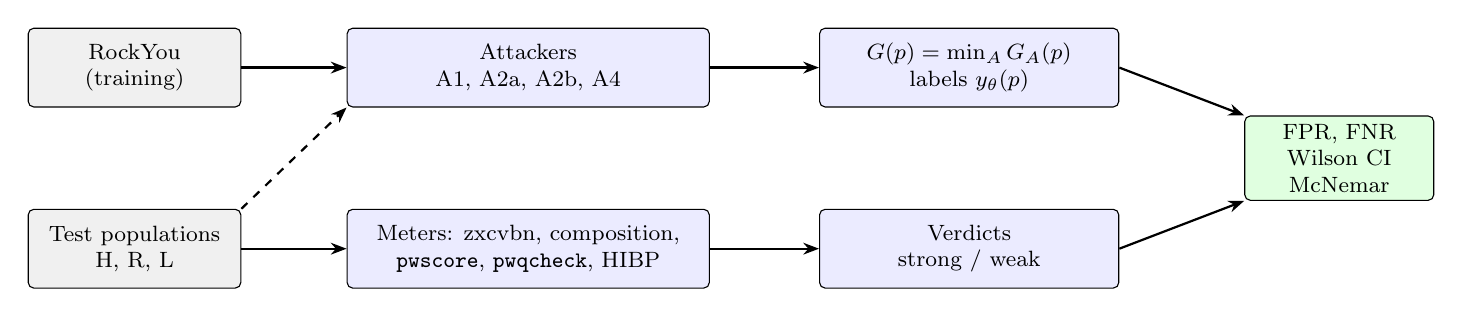
\begin{tikzpicture}[
  box/.style={draw, rounded corners=2pt, align=center, font=\footnotesize, minimum height=10mm, inner sep=3pt},
  dat/.style={box, fill=gray!12},
  prc/.style={box, fill=blue!8},
  res/.style={box, fill=green!12},
  arr/.style={-{Stealth[length=2mm]}, thick}]
\node[dat, minimum width=27mm] (train) at (0,0) {RockYou\\ (training)};
\node[prc, minimum width=46mm] (att) at (5.0,0) {Attackers\\ A1, A2a, A2b, A4};
\node[prc, minimum width=38mm] (gt) at (10.6,0) {$G(p)=\min_A G_A(p)$\\ labels $y_\theta(p)$};
\node[dat, minimum width=27mm] (pop) at (0,-2.3) {Test populations\\ H, R, L};
\node[prc, minimum width=46mm] (met) at (5.0,-2.3) {Meters: zxcvbn, composition,\\ \texttt{pwscore}, \texttt{pwqcheck}, HIBP};
\node[prc, minimum width=38mm] (ver) at (10.6,-2.3) {Verdicts\\ strong / weak};
\node[res, minimum width=24mm] (out) at (15.3,-1.15) {FPR, FNR\\ Wilson CI\\ McNemar};
\draw[arr] (train) -- (att);
\draw[arr] (att) -- (gt);
\draw[arr] (pop) -- (met);
\draw[arr] (met) -- (ver);
\draw[arr, dashed] (pop.north east) -- (att.south west);
\draw[arr] (gt.east) -- (out.north west);
\draw[arr] (ver.east) -- (out.south west);
\end{tikzpicture}
\caption{Evaluation pipeline. Attackers are trained on RockYou (and, for A4, on L-train) and guess the test populations (dashed); meters score the same passwords; both outputs meet in the error metrics.}
\label{fig:pipeline}
\end{figure*}


\begin{table}[t]
\centering
\caption{Design decisions and their sources.}
\label{tab:decisions}
\footnotesize
\renewcommand{\arraystretch}{1.12}
\begin{tabularx}{\columnwidth}{@{}Y Y@{}}
\toprule
\textbf{Decision} & \textbf{Source}\\
\midrule
Ground truth = minimum over several attackers & Ur 2015~\cite{ur2015}; Wheeler~\cite{wheeler2016}; Wang~\cite{wang2023}\\
Attackers trained on a service other than the test service & Wang~\cite{wang2023}; Wheeler's caveat~\cite{wheeler2016}\\
Observations weighted by account frequency & Golla~\cite{golla2018}\\
Online budgets $10^4$, $10^6$ & Wang~\cite{wang2023}; Flor\^encio~\cite{florencio2016}; Tan~\cite{tan2020}; Golla~\cite{golla2018}\\
Offline-style budget $B=10^{10}$ & zxcvbn score 4; GPU rates in~\cite{golla2018}; our measured rate\\
One-sided error (strong rate among guessed) & Wang's weak$\to$strong argument~\cite{wang2023}; limitation noted in~\cite{golla2018}\\
HIBP verdict on the entire password & NIST blocklist rule~\cite{nist80063b4}\\
Minimum length 8; blocklist verdict without composition rules & NIST~\cite{nist80063b4}\\
Meters binned to accept/reject, plus threshold sweeps & Golla on quantization~\cite{golla2018}; Wang on binning~\cite{wang2023}\\
\bottomrule
\end{tabularx}
\end{table}

%% =====================================================================
\section{Feasibility and Action Plan}\label{sec:feasibility}

\subsection{Pilot measurements}
We measured the components on a reference machine (2 vCPU, 7~GB RAM, not the team VMs); Table~\ref{tab:pilot} gives the results. A $10^{10}$-guess stream is feasible in under an hour, and the meters process $10^5$ passwords in minutes. Two more checks were possible. A Pwned Passwords range query for the prefix \texttt{5BAA6}, made through a web-fetch tool because the shell could not reach the API, returned the list of SHA-1 suffixes with counts without any key, including the suffix of ``password'' (52{,}372{,}427 occurrences on 30 Oct. 2026)~\cite{hibp}. And the zxcvbn Python port matches the JavaScript reference once its reference year is aligned (see below). The LLM generation speed could not be measured here (model registries were unreachable); Sec.~\ref{sec:zerocost} bounds it and week~1 measures it.

\begin{table}[t]
\centering
\caption{Pilot measurements on the reference machine.}
\label{tab:pilot}
\footnotesize
\renewcommand{\arraystretch}{1.12}
\begin{tabularx}{\columnwidth}{@{}Y r@{}}
\toprule
\textbf{Measurement} & \textbf{Result}\\
\midrule
zxcvbn (Python), passwords per second & 2{,}049\\
\texttt{pwscore} / \texttt{pwqcheck}, calls per second & 539 / 640\\
hashcat \texttt{dive} stream into a Python consumer, candidates per second & $4.06{\times}10^{6}$\\
\quad (198{,}172{,}317 candidates in 48.8 s) & \\
hashcat \texttt{best64} on 200\,k words, candidates per second & $5.9{\times}10^{5}$\\
Unique / total candidates for 40 random top-20\,k RockYou words: \texttt{best64}, \texttt{T0XlCv2}, \texttt{d3ad0ne}, \texttt{dive} & 0.945, 0.734, 0.589, 0.492\\
Time for $10^{9}$, $10^{10}$, $10^{11}$, $10^{14}$ candidates at $4.06{\times}10^{6}$/s & 4 min, 41 min, 6.8 h, 285 d\\
\bottomrule
\end{tabularx}
\end{table}

The duplicate ratio shows that raw stream positions overstate the deduplicated rank by up to a factor $\approx2$ (0.3 orders of magnitude) for \texttt{dive}; we keep raw positions (what a naive attacker pays) and run a deduplicated variant on a sample as a robustness check.

\textbf{Sanity checks.} We recomputed the formulas independently: the Wilson interval (Eq.~\ref{eq:wilson}) against \texttt{statsmodels}; Eq.~\eqref{eq:wsp} against SciPy's Spearman coefficient on account-level data (difference below $10^{-16}$), which also shows that the classical $1-6\sum d^2/(n(n^2-1))$ formula is invalid with ties; the zxcvbn thresholds of Eq.~\eqref{eq:zxscore}; and the Monte Carlo rank estimator of~\cite{dellamico2015} on a toy Markov model of 97{,}655 strings with exact ranks (200 repetitions of $10^4$ samples: bias below 0.3\,\% and relative standard deviation of about 2-3\,\% up to rank $10^4$, but 138\,\% at rank 90{,}000 of 97{,}655). The estimator is therefore kept as future work, not as part of the ground truth.

\textbf{zxcvbn parity.} We compared the Python port with the JavaScript reference (npm version 4.4.2) on 3{,}012 passwords: 3{,}000 drawn at random from phpBB with a fixed seed and 12 hand-picked strings. As shipped, the two disagree on the guess estimate of 280 passwords (9.3\,\%, up to 47\,\% relative difference) and on the score of 3 (0.1\,\%). The cause is the reference year used for date patterns: the Python port fixes \texttt{REFERENCE\_YEAR} at 2017, whereas the JavaScript code uses the current year. With the year set to 2026 in Python, the outputs agree on all 3{,}012 passwords (relative difference below $10^{-15}$). Our wrapper therefore pins the year, which also makes the results independent of the date of the run.

\subsection{End-to-end smoke test}
To check the whole pipeline, we ran the four locally available meters on H against attacker A1 alone (Table~\ref{tab:smoke}). A1 guesses 12{,}099 of 116{,}289 accounts (10.4\,\%) within $10^4$ guesses and 34{,}803 (29.9\,\%) within $10^6$; its whole list ($1.4{\times}10^7$ guesses) contains 44{,}846 accounts (38.6\,\%). This is not a result of the study: A2, A4 and the full set of populations are missing, so FPR is expected to be a lower bound and FNR to be inflated. It shows two things. The meters differ mainly in strictness (strong rate from 4.5\,\% to 63.0\,\%), so FPR alone would reward a meter that rejects everything, which justifies reporting FNR and curves. And a dictionary alone is not enough: variants such as capitalized or digit-suffixed words are the ones that can pass composition rules, which is why A2 is part of the protocol~\cite{ur2015}.

\begin{table}[t]
\centering
\caption{Smoke test: attacker A1 only, H (116{,}289 accounts, phpBB, $\ge8$ chars). Wilson half-widths are at most 0.5 points. Strong rate is over all accounts.}
\label{tab:smoke}
\footnotesize
\renewcommand{\arraystretch}{1.12}
\setlength{\tabcolsep}{4pt}
\begin{tabular}{@{}l r r r r@{}}
\toprule
\textbf{Meter} & \textbf{Strong rate} & \textbf{FPR $10^4$} & \textbf{FPR $10^6$} & \textbf{FNR $10^6$}\\
\midrule
zxcvbn (score $\ge3$) & 15.3\,\% & 0.1\,\% & 2.5\,\% & 79.3\,\%\\
Composition & 7.6\,\% & 0.1\,\% & 0.5\,\% & 89.4\,\%\\
\texttt{pwscore} (accepted) & 63.0\,\% & 7.1\,\% & 25.6\,\% & 21.0\,\%\\
\texttt{pwqcheck} (accepted) & 4.5\,\% & 0.0\,\% & 0.0\,\% & 93.6\,\%\\
\bottomrule
\end{tabular}
\end{table}

\subsection{Zero-cost resources}\label{sec:zerocost}
The project must cost nothing: no paid API, no new subscription, no rented machine. Table~\ref{tab:cost} lists each resource. The only paid assets the team already holds are a Claude Pro and a Gemini student subscription, and the pipeline does not depend on either. Claude Pro does not include API access, which is billed separately~\cite{claudebilling}, so Claude models can enter only through a small manual sample.

\textbf{LLM generation costs time, not money.} For one sequence, each decoded token reads the whole quantised model from memory, so the speed is at most the memory bandwidth divided by the model size. Dual-channel DDR4-3200 gives $3200\times10^6\times8\times2=51.2$~GB/s; the default Llama~3.2 3B build is 2.0~GB~\cite{ollama}, hence at most $25.6$ tokens/s, whereas a 7B-class model (about 4~GB) is capped near 13 tokens/s. We therefore restrict the models to 4~billion parameters. The population needs $3\text{ models}\times2\text{ prompts}\times2\text{ sets}\times1{,}000=12{,}000$ generations. Charging 50 prompt tokens and a 64-token answer cap to every generation at the decoding speed, one generation takes $114/v$~s: the 12{,}000 generations need 19 machine-hours at $v=20$ tokens/s and 38 at $v=10$, i.e.\ 4.8 or 9.5 hours per machine on four team laptops, run overnight. The week-1 gate measures $v$ on each laptop; below 10 tokens/s, we cut $N$ to 500 or use two models.

\textbf{Optional external-validity samples.} (i)~The Gemini API has a free tier without credit card for Flash models~\cite{geminipricing}; a request is billed only if its project is linked to an active billing account~\cite{geminiterms}, so we would never link one. Free-tier content may be used to improve Google products and read by reviewers~\cite{geminiterms}, which is harmless here since we send a generation prompt and no real password; its limits are shown in Google AI Studio and are not guaranteed, so it is used only if the quota suffices. (ii)~Fifty generations per assistant (the number of runs in~\cite{irregular2026}) typed by hand in new conversations of the Claude Pro and Gemini chat applications, never scripted. These samples feed only the duplicate-rate and verdict comparison, not attacker A4.

\begin{table}[t]
\centering
\caption{Resources and their cost.}
\label{tab:cost}
\footnotesize
\renewcommand{\arraystretch}{1.12}
\begin{tabularx}{\columnwidth}{@{}l Y Y@{}}
\toprule
\textbf{Resource} & \textbf{Role} & \textbf{Cost}\\
\midrule
SecLists leaks~\cite{seclists} & H, attacker training & free, public\\
hashcat~\cite{hashcat} & attackers A2a, A2b & free\\
zxcvbn, \texttt{libpwquality}, \texttt{passwdqc} & meters & free (installed in the pilot)\\
HIBP range API~\cite{hibp} & meter & free, no key\\
Ollama, 3 open-weight models $\le4$~B & L population & free, local CPU\\
Gemini API free tier & optional sample & free without billing account\\
Claude Pro, Gemini chat & optional manual samples & already owned, no extra\\
Team laptops / VMs & all computation & no cloud rental\\
GitHub, local \LaTeX & repository, report & free\\
\bottomrule
\end{tabularx}
\end{table}

\subsection{Nine-week plan}
Table~\ref{tab:plan} gives the plan. Compute is not the bottleneck: both attack streams take about 1.2 hours, and the meters about 4 minutes on H (smoke test: about 40 s for zxcvbn and about 160 s for the two Linux tools with two processes). The main remaining risk is LLM generation time, which has a week-1 gate; the HIBP access and the zxcvbn parity were tested in the pilot.

\begin{table}[t]
\centering
\caption{Nine-week plan.}
\label{tab:plan}
\footnotesize
\renewcommand{\arraystretch}{1.12}
\begin{tabularx}{\columnwidth}{@{}c Y@{}}
\toprule
\textbf{Wk} & \textbf{Work and deliverable}\\
\midrule
1 & Machines, repository skeleton; \textbf{gates}: LLM throughput benchmark on each laptop ($\ge10$ tokens/s, else $N=500$ or two models), HIBP test with 100 passwords from a team machine; zxcvbn parity kept as a unit test\\
2 & Data filters, meter wrappers with \texttt{pytest}; verdict table for H\\
3 & Attackers A1, A2a, A2b: streaming consumer, deduplicated sample; $G(p)$ for H\\
4 & LLM generation (batched), A4, random control R\\
5 & Full run: all meters $\times$ populations; HIBP lookups with prefix cache; master table\\
6 & Metrics: FPR, FNR, Wilson, McNemar, threshold sweeps; figures\\
7 & Robustness: HIBP contamination of H, deduplication effect, weighted Spearman; optional Markov/Monte Carlo\\
8 & Part~2 report, README, \texttt{Makefile} reproducing every table\\
9 & Buffer, review, presentation\\
\bottomrule
\end{tabularx}
\end{table}

\subsection{Repository and ethics}
The repository, to be created at the start of the practical part, will contain \texttt{src/meters}, \texttt{src/attackers}, \texttt{src/llm}, \texttt{src/metrics}, \texttt{tests/}, \texttt{results/} (aggregated counts only), \texttt{paper/} and a \texttt{Makefile}; library versions are pinned. We use only public leaks distributed in SecLists~\cite{seclists}, keep raw leak files on the VMs and out of the repository, do not try to identify individuals, send only five-hex-character SHA-1 prefixes to HIBP~\cite{hibp}, and publish no credential. No paid service is used: no billed API key and no cloud rental (Sec.~\ref{sec:zerocost}).

%% =====================================================================
\section{Threats to Validity}
\begin{itemize}
\item \textbf{Ground truth.} Our attackers are weaker than the best ones and capped at $10^{10}$; FPR are expected to be lower bounds. Raw stream positions over-state guess numbers by up to $\approx2\times$.
\item \textbf{Data.} One test leak (phpBB), English-speaking users, one training leak (RockYou). Both leaks reflect their own service and policy~\cite{golla2018}. Robustness with a second test leak is optional.
\item \textbf{HIBP circularity.} The leaks may be part of HIBP, as Golla and D\"urmuth observe for their own data~\cite{golla2018}. We measure the contamination of H in week~7 and read HIBP chiefly on R and L.
\item \textbf{LLM population.} Results depend on the models, prompts, temperature and versions; the free, local models of at most 4~B parameters may differ from the commercial assistants studied in~\cite{irregular2026}; the optional manual samples check whether the duplicate rate carries over. A4 is a strong attacker that knows the model.
\item \textbf{Implementation.} We use the zxcvbn Python port rather than the JavaScript reference of~\cite{wheeler2016,golla2018}; the two agree on 3{,}012 passwords once the reference year is pinned, but only that sample was compared. Default configurations of the Linux tools are fixed in the repository.
\item \textbf{Thresholds.} Budgets above $10^6$ lie in the ``don't care'' region of~\cite{florencio2016}; results at $10^8$-$10^{10}$ test a meter's own scale rather than a modeled attack.
\end{itemize}

%% =====================================================================
\section{Conclusion and Future Work}
We reviewed eight related works, identified a gap (one-sided error rates of binary verdicts, Linux password-quality tools, LLM passwords with an LLM-aware attacker) and specified a protocol whose design is justified by the literature and whose feasibility is supported by measurements. The plan fits in nine weeks, uses only free resources, and the first end-to-end run already shows why both FPR and FNR are needed. The practical part will report the results, starting with the five meters on H, R and L at $\theta_{\text{on}}=10^6$ and $\theta_{\text{off}}=10^{10}$.

\emph{Future work.} Three extensions follow from the limits above: stronger ground-truth attackers (Markov or PCFG models, and the Monte Carlo rank estimator of~\cite{dellamico2015} once its variance at high ranks is controlled); a second test leak, to measure the dependence on the service; and LLM samples from larger or commercial models, together with targeted attackers that use profile data as in~\cite{atzori2025}.

\bibliographystyle{IEEEtranHY}
\bibliography{refs}

\end{document}
